\documentclass[journal,comsoc]{IEEEtran}
\usepackage[T1]{fontenc}
\usepackage{graphicx}
\usepackage{adjustbox}
\usepackage{cite}
\usepackage{float}
\usepackage[T1]{fontenc}% optional T1 font encoding
\usepackage{etoolbox}
\makeatletter
\patchcmd{\@makecaption}
  {\scshape}
  {}
  {}
  {}
\makeatletter
\patchcmd{\@makecaption}
  {\\}
  {.\ }
  {}
  {}
\makeatother
\def\tablename{Table}

\ifCLASSINFOpdf
  % \usepackage[pdftex]{graphicx}
  % declare the path(s) where your graphic files are
  % \graphicspath{{../pdf/}{../jpeg/}}
  % and their extensions so you won't have to specify these with
  % every instance of \includegraphics
  % \DeclareGraphicsExtensions{.pdf,.jpeg,.png}
\else
  % or other class option (dvipsone, dvipdf, if not using dvips). graphicx
  % will default to the driver specified in the system graphics.cfg if no
  % driver is specified.
  % \usepackage[dvips]{graphicx}
  % declare the path(s) where your graphic files are
  % \graphicspath{{../eps/}}
  % and their extensions so you won't have to specify these with
  % every instance of \includegraphics
  % \DeclareGraphicsExtensions{.eps}
\fi

\usepackage{amsmath}
\interdisplaylinepenalty=2500
\usepackage[cmintegrals]{newtxmath}
\usepackage{algorithmic}

\ifCLASSOPTIONcaptionsoff
  \usepackage[nomarkers]{endfloat}
 \let\MYoriglatexcaption\caption
 \renewcommand{\caption}[2][\relax]{\MYoriglatexcaption[#2]{#2}}
\fi

% Untuk memperbaiki pemenggalan kata yang salah.
% \hyphenation{op-tical net-works semi-conduc-tor}

\title{Water quality prediction of Lake Toba using Extreme Learning Machine (ELM)}
\author{
	\IEEEauthorblockN{Romi~Fadillah~Rahmat, Eric~Suwarno, and Maya~Silvi~Lydia}
	\\
    \IEEEauthorblockA{Faculty~of~Computer~Science~and~Information~Technology
    \\University~of~Sumatera~Utara
    \\Medan,~Indonesia
    \\romi.fadillah@usu.ac.id, 121402071.es@gmail.com, maya2@usu.ac.id
	}
}

\begin{document}

\markboth{}%
{Water quality prediction of Lake Toba using Extreme Learning Machine (ELM)}

\maketitle

\begin{abstract}

% Abstrak

Currently, the pollution level occurred in Lake Toba varies from lightly polluted to slightly higher level. Thus, there is an increase of the necessity to manage environmental quality of Lake Toba, especially the water quality. Currently, the water quality assessment is done over the laboratory test by obtaining the sample on selected locations of Lake Toba. While Rahmat \textit{et al.} \cite{Rahmat16} proposed a real-time assessment of water quality in Lake Toba, a method should be implemented to predict the water quality of Lake Toba based on the data collected from the assessment process. In this research, extreme learning machine (ELM) is implemented to predict water quality in Lake Toba. Compared to the backpropagation algorithm, the result shows that the water quality prediction done by using extreme learning machine ...

\end{abstract}

\begin{IEEEkeywords}

extreme learning machines (ELM), water quality, Lake Toba, artificial neural networks.

\end{IEEEkeywords}

\section{Introduction}

% Pendahuluan

According to Haro \textit{et al.} \cite{Haro13}, the pollution has been occurred in Lake Toba in North Sumatera province, Indonesia. The level of pollution in Lake Toba varies from lightly polluted to medium level pollution. Residential waste, along with the industrial waste and water hyacinth population on the lake surface, are the main source of the water pollution in Lake Toba.

The water quality assessment is performed by obtaining the sample from several locations around the coastline of Lake Toba. Each samples will be examined by laboratory test to determine the water quality status of Lake Toba. As this assessment method takes more time to be performed, along with the cost of assessment, a method has to be implemented to reduce the time and the cost of assessment process.

The vast development of information technology has enabled 

\section{Theoretical background}

% Landasan Teori

\subsection{Extreme learning machine}

According to Sun \textit{et al.} \cite{Gao14}, extreme learning machines (ELM) refers to a learning method applied in artificial neural networks. The architecture of neural network utilized in extreme learning machine is single hidden layer feedforward neural networks.

Extreme learning machines is proposed by Huang \textit{et al.} \cite{Huang06} to increase the calculation speed of artificial neural networks, by randomizing the hidden layer. They stated that the feedforward neural network utilizes slow gradient based learning, which results in longer computational time. The randomization of the hidden layer results in faster computational speed, along with higher processing result accuracy.

A single hidden layer feed-forward neural network is defined by \eqref{Eq. 1}:

\begin{equation}
f_{n} (x) = \sum_{i=1}^{n} G_{i} (x, a_{i}, b_{i}) * \beta_{i}, a_{i} \in R^d, b_{i}, \beta_{i} \in R\label{Eq. 1}
\end{equation}

where $G_{i}(\cdot)$ refers to the activation function calculated in the ith hidden neuron, $a_{i}$ refers to the input weight received by the ith hidden neuron from input neuron, $b_{i}$ refers to the bias weight of the hidden neuron, and $\beta_{i}$ refers to output weight of the hidden neuron.

For each additional nodes, $G_{i}$ is defined from the additional node activation function $g$, as described by \eqref{Eq. 2}:

\begin{equation}
G_{i} (x, a_{i}, b_{i}) * \beta_{i} = g(a_{i} \times x + b_{i})\label{Eq. 2}
\end{equation}

Equation \eqref{Eq. 3} is implemented when the hidden neuron implements RBF as the activation function.

\begin{equation}
G_{i}(x, a_{i}, b_{i}) * \beta_{i} = g(b_{i}\parallel x - a_{i} \parallel)\label{Eq. 3}
\end{equation}

Suppose a training data set $ N = \{(x_{i},t_{i}) \mid x_{i} \in R_{n}, t_{i} \in R_{m}, i = 1, ..., L\}$, with $x_{i}$ represents the training data, $t_{i}$ represents the class label of the sample for each instance, and $L$ is defined as the number of hidden nodes. When implementing the extreme learning machine for training the neural network, the steps are done as follows:

\begin{itemize}
\item Assign input weights $w_{i}$ and biases $b_{i}$, where $i = 1, ..., L$,
\item Calculate the hidden layer output matrix as H,
\item Calculate the output weight, as defined in \eqref{Eq. 4}:
\begin{equation}
\beta = H^\dagger T\label{Eq. 4}
\end{equation}
where $T = [t_{1},...,t_{N}]^T$ and $H^\dagger$ refers to the Moore-Penrose inverse of matrix $H$.
\end{itemize}

\subsection{Water quality index}



\section{Methodology}

% Metodologi
This section describes the methodology of this research. The general architecture is shown by Figure 1.

\begin{figure}[th]
	\centering
	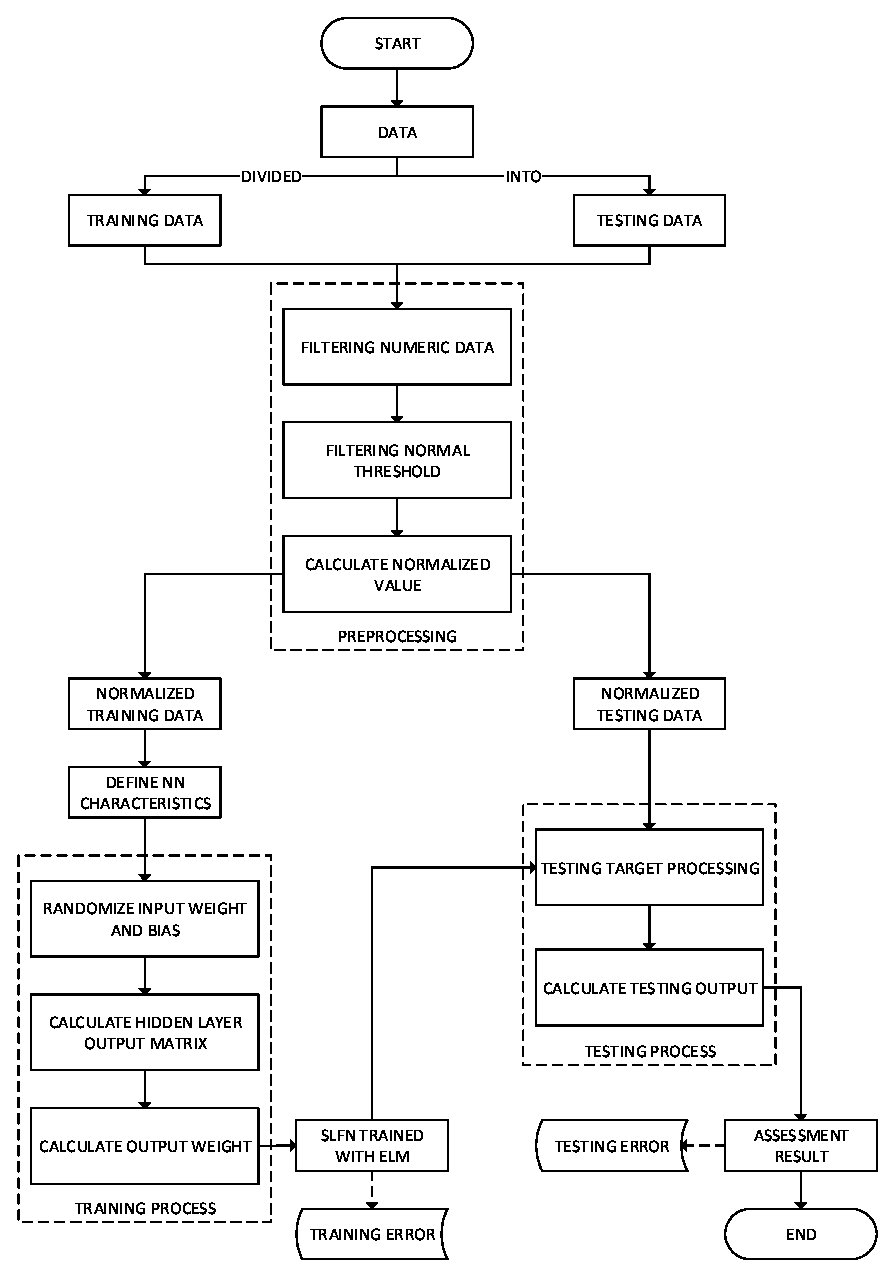
\includegraphics[height=8cm]{ArsitekturUmum-Redesigned-Remastered.eps}
	\caption{General architecture of the research}
\end{figure}

The steps performed in this research are described as follows:

\begin{enumerate}
	\item Data input: The data utilized in this research is obtained from the research done by Rahmat et al. \cite{Rahmat16}, with the format shown by Figure 2. Each data file will be split into two datasets, namely training dataset and testing dataset, with the ratio of 60:40.
	
	\begin{figure}[th]
		\centering
		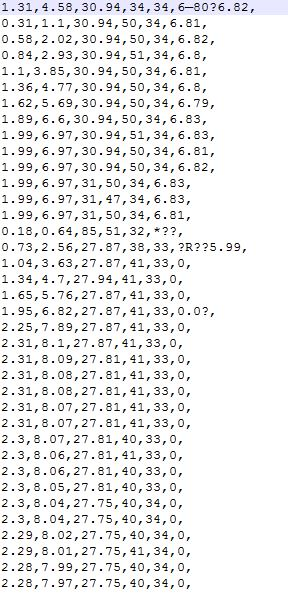
\includegraphics[width=0.8\columnwidth, height=5cm]{initial-structure.jpg}
		\caption{Initial structure of the data}
	\end{figure}
	
	\item Preprocessing: Each training and testing dataset will be preprocessed in order to enable the data to be processed by extreme learning machine. The process is performed in three steps, described as follows:
	
	\begin{itemize}
		\item Filtering each row to ensure that each dataset contains fully numeric value;
		\item Filtering each row to ensure that contains the normal value of measurement; and
		\item Calculating the normalized value of each parameter, which is done by using Eq. 5:
		
		\begin{equation}
		A' = \frac{A - A_{min}}{A_{max} - A_{min}} * (D - C) + C\label{Eq. 5}
		\end{equation}
	\end{itemize}

    
\end{enumerate}

\section{Experiment and Result}

% Implementasi dan Hasil

\section{Conclusion}

% Kesimpulan

\ifCLASSOPTIONcaptionsoff
  \newpage
\fi

\begin{thebibliography}{1}

\bibitem{Rahmat16}
R. F. Rahmat, Athmanathan, M. F. Syahputra dan M. S. Lydia, \textquotedblleft 
	Real Time Monitoring System for Water Pollution in Lake Toba,\textquotedblright \ in
	{\it Proceedings of ICIC 2016}, Lombok, 2016.

\bibitem{Haro13}
D.~D.~Haro, Y.~Djayus and Z.~Harahap, \textquotedblleft Kondisi Kualitas Air
  Danau Toba di Kecamatan Haranggaol Horison Kabupaten Simalungun Sumatera
  Utara\textquotedblright , {\it AQUACOASTMARINE}, vol. 1, no. 1, 2013.
  
\bibitem{Gao14}
M.~Gao, W.~Xu, H.~Fu, M.~Wang and X.~Liang, \textquotedblleft A Novel Forecasting 
	Method for Large-Scale Sales Prediction Using Extreme Learning Machine,
	\textquotedblright \hskip 1em plus 0.5em minus 0.4mm\relax 
	{\it 2014 Seventh International Joint Conference on Computational Sciences and Optimization},
	Beijing, 2014, pp. ~602--606.

\bibitem{Huang06}
G.-B.~Huang, Q.-Y.~Zhu, and C.-K.~Siew, \textquotedblleft Extreme
  learning machine: Theory and applications,\textquotedblright \hskip 1em plus
  0.5em minus 0.4mm\relax \ {\it Neurocomputing}, vol. 70, no. 1-3, pp. ~489--501, Dec. 2006.

\end{thebibliography}

\end{document}
